	\large \bf{\textsc{\section{Lab 1}}
	\begin{problem}
		Choose a 15K\(\Omega\) resistor. Read the color code and tolerance.
		\newline
		1. Measure the resistance using a multimeter.
		\newline
		2. Adjust the power supply on 5V. Connect the resistors to the power supply. Measure the voltage and the current of the resistor.
		\newline
		3. Repeat step two for 11 different voltages ranging from -15V to 15V.
		\newline
		4. Plot the I-V characteristics of the resistors. Are all measurements on one line? What is the slope of the line? Compare it with your readings of the code and tolerance as well as the multimeter readings. 
	\end{problem}

	\begin{solution}
		1. We measured the resistor to be 14.93K\(\Omega\).
		\newline
		2.Voltage: 5.15V and Amperage: 0.35 mA 
		\newline
		3. 
		\begin{table}[h]
			\begin{tabular}{| l | l | l | l | l | l | l | l | l | l | l | l |}
				\hline
				\textbf{Try} & 1 & 2 & 3 & 4 & 5 & 6 & 7 & 8 & 9 & 10 & 11 \\ \hline
				Voltage (V)  & -14.98 & -12.82 & -9.19 & -7.19 & -3.66 & 2.25 & 4.30 & 6.92 & 9.57 & 12.46 & 15 \\ \hline
				Current (mA) & -1.01 & -0.86 & -0.62 & -0.42 & -0.25 & 0.15 & 0.29 & 0.47 & 0.64 & 0.84 & 1.01 \\ \hline
			\end{tabular}
		\end{table}
		\newline
		4. 
		\begin{figure}[h!]
			\centering
			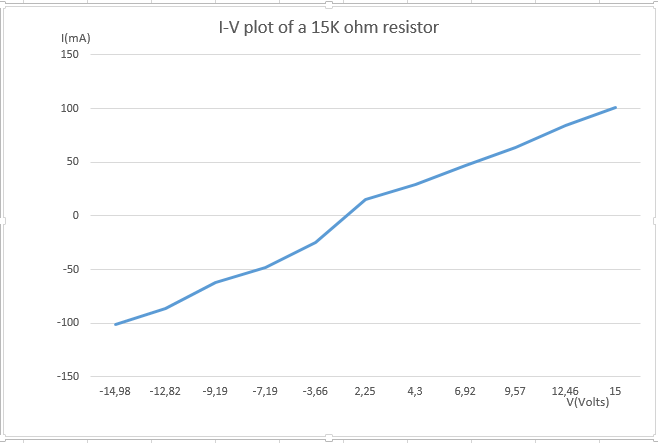
\includegraphics[width=0.5\textwidth]{images/ivplot.png}
		\end{figure}
	
		
	\end{solution}
	The slope is:
		$ (47 mA-29 mA)/(6.92 V-4.3 V)=6.87 mA/V $
	\clearpage
	\begin{problem}
		Choose the following resistors and construct each circuit given in the figure. \\
		R\(_{1}\): 15K\(\Omega\) \\
		R\(_{2}\): 22K\(\Omega\) \\
		R\(_{3}\): 33K\(\Omega\) \\
		R\(_{4}\): 10K\(\Omega\) \\
		\newline
		1. Calculate the equivalent resistance.
		\newline
		2. Measure the resistance of each indicated terminal using multimeter.
		\newline
		3. Are they different? Check out the tolerances and conclude why there is a difference.
		\begin{figure}[h!]
			\centering
			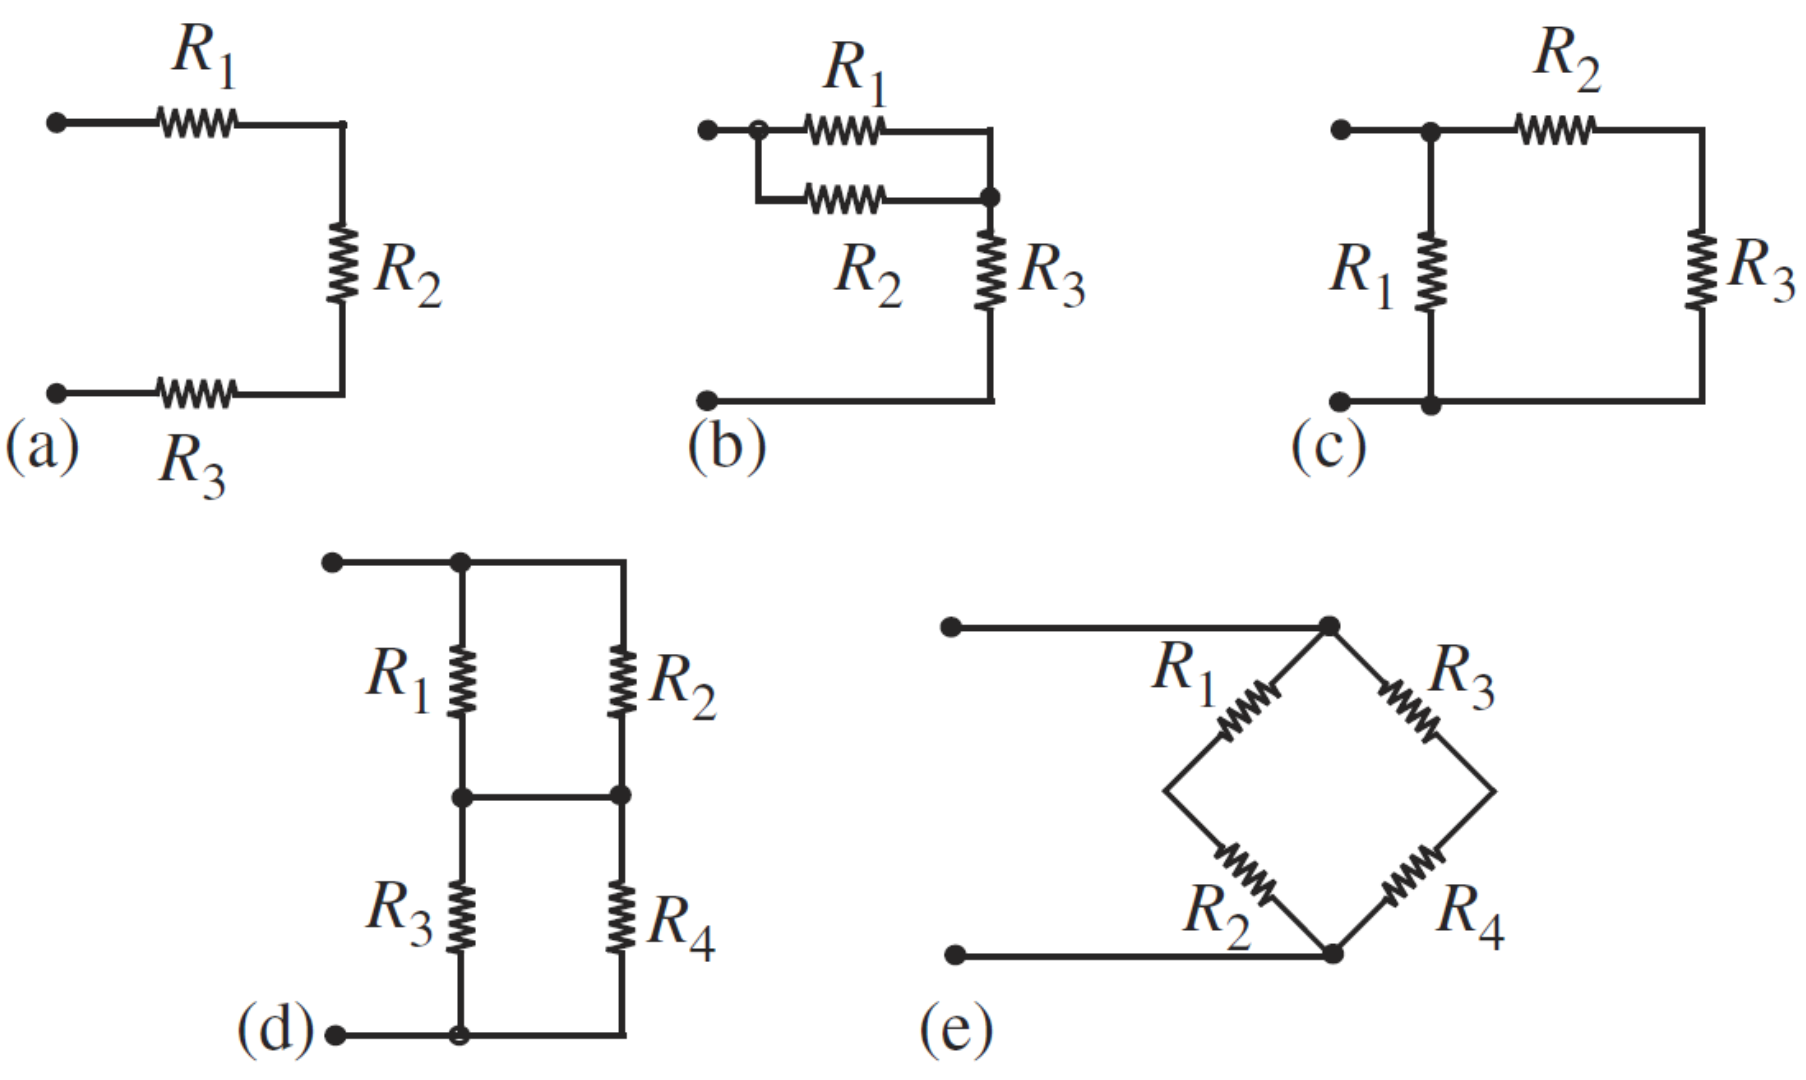
\includegraphics[width=0.5\textwidth]{images/figure1.png}
		\end{figure}
	\end{problem}
	
	\begin{solution}
		1. 
		(a) resistance is 70K\(\Omega\) \\
		(b) resistance is 41.91K\(\Omega\) \\
		(c) resistance is 11.78K\(\Omega\) \\
		(d) resistance is 16.59K\(\Omega\) \\
		(e) resistance is 19.88K\(\Omega\) \\
		\newline
		2. 
		(a) resistance is 69.8K\(\Omega\) \\
		(b) resistance is 41.7K\(\Omega\) \\
		(c) resistance is 11.73K\(\Omega\) \\
		(d) resistance is 16.55K\(\Omega\) \\
		(e) resistance is 19.8K\(\Omega\) \\
		\newline
		3. The average difference between measurements is (0.28+0.48+0.42+0.24+0.4)/5=0.36 percent. This is well within the 1 percent error the resistors are given for.
	\end{solution}
	\clearpage
	\begin{problem}
		Construct the circuit given in the following figure.
		\newline
		V\(_{A}\): 5V \\
		V\(_{B}\): 10V \\
		R\(_{1}\): 22K\(\Omega\) \\
		R\(_{2}\): 33K\(\Omega\) \\
		R\(_{3}\): 10K\(\Omega\) \\
		\newline
		1. Find all voltages and currents using KVL and KCL method.
		\newline
		2. Measure all currents and voltages stated in the circuit.
		\newline
		3. Compare the results.
		\begin{figure}[h!]
			\centering
			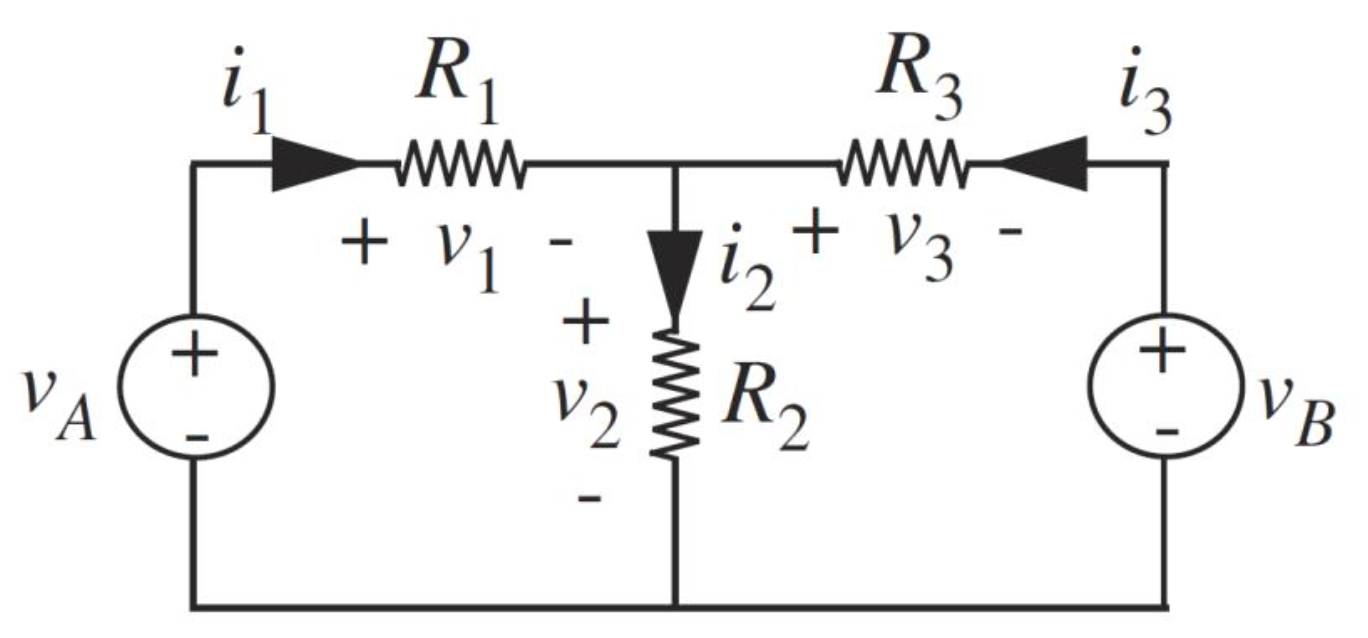
\includegraphics[width=0.2\textwidth]{images/circuit5.png}
		\end{figure}
	\end{problem}
	
	\begin{solution}
		\begin{figure}[h!]
				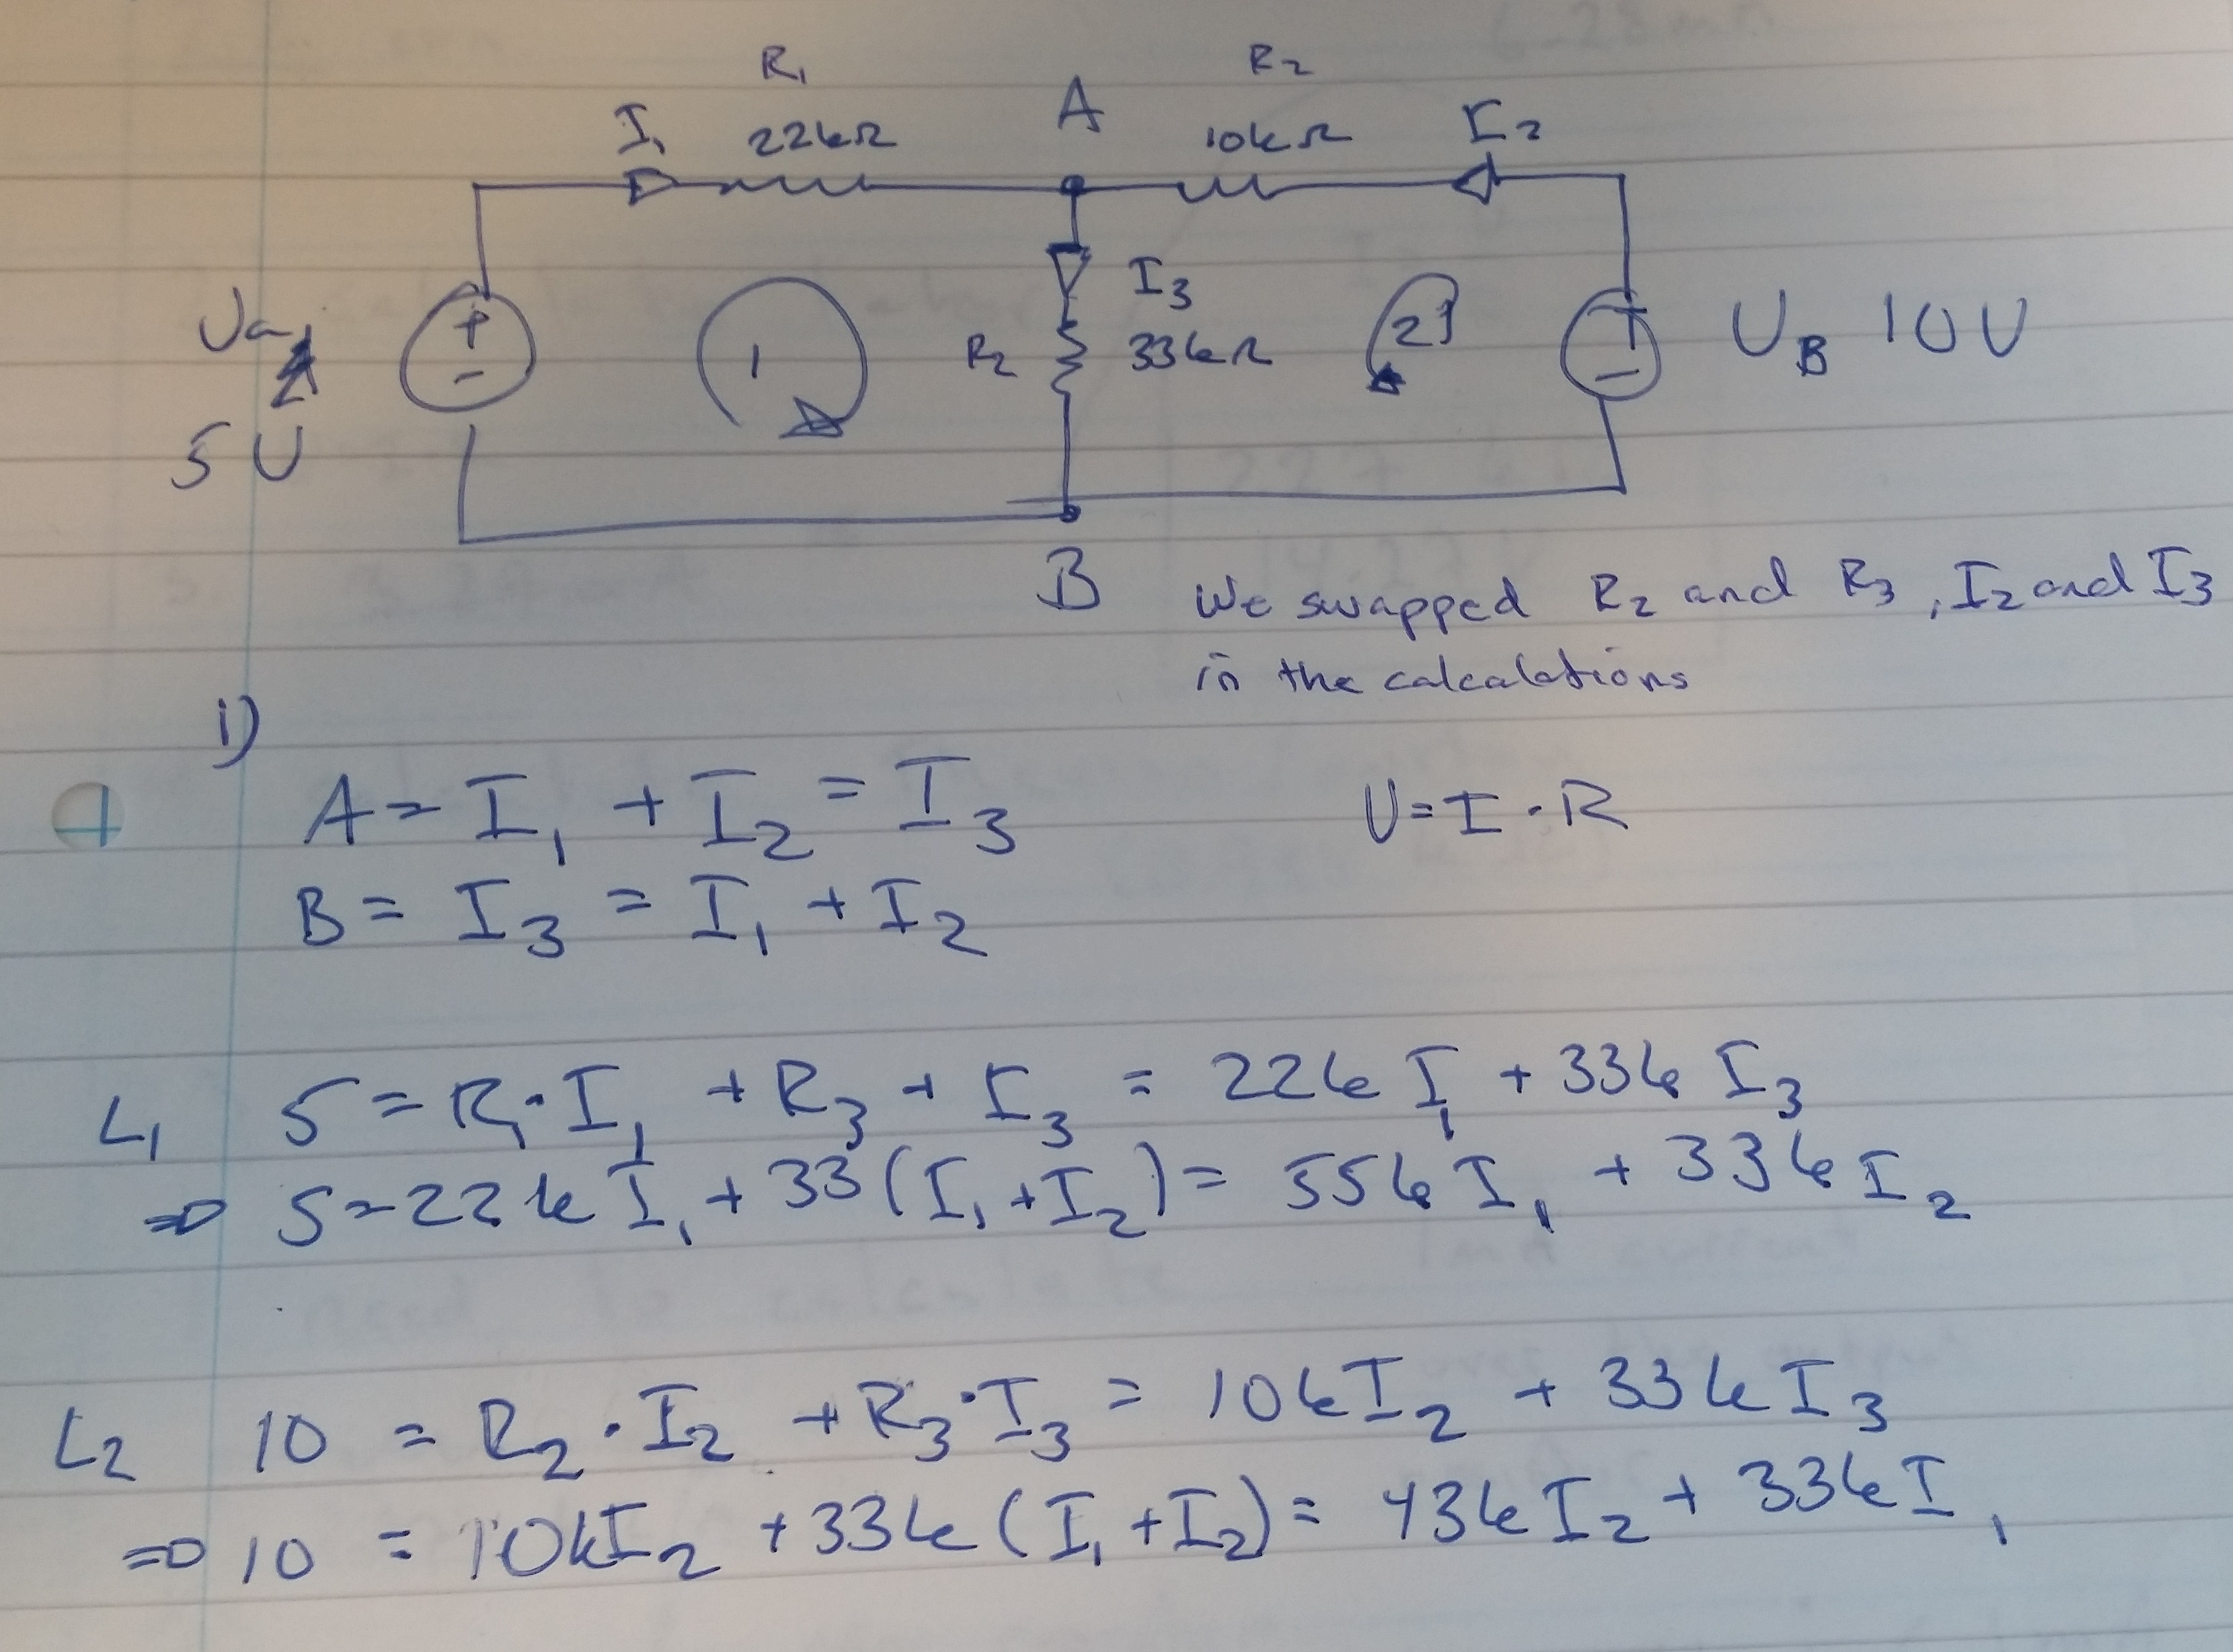
\includegraphics[width=0.6\textwidth]{images/lab1pic1.jpg}
		\end{figure}
		\begin{figure}[h!]
				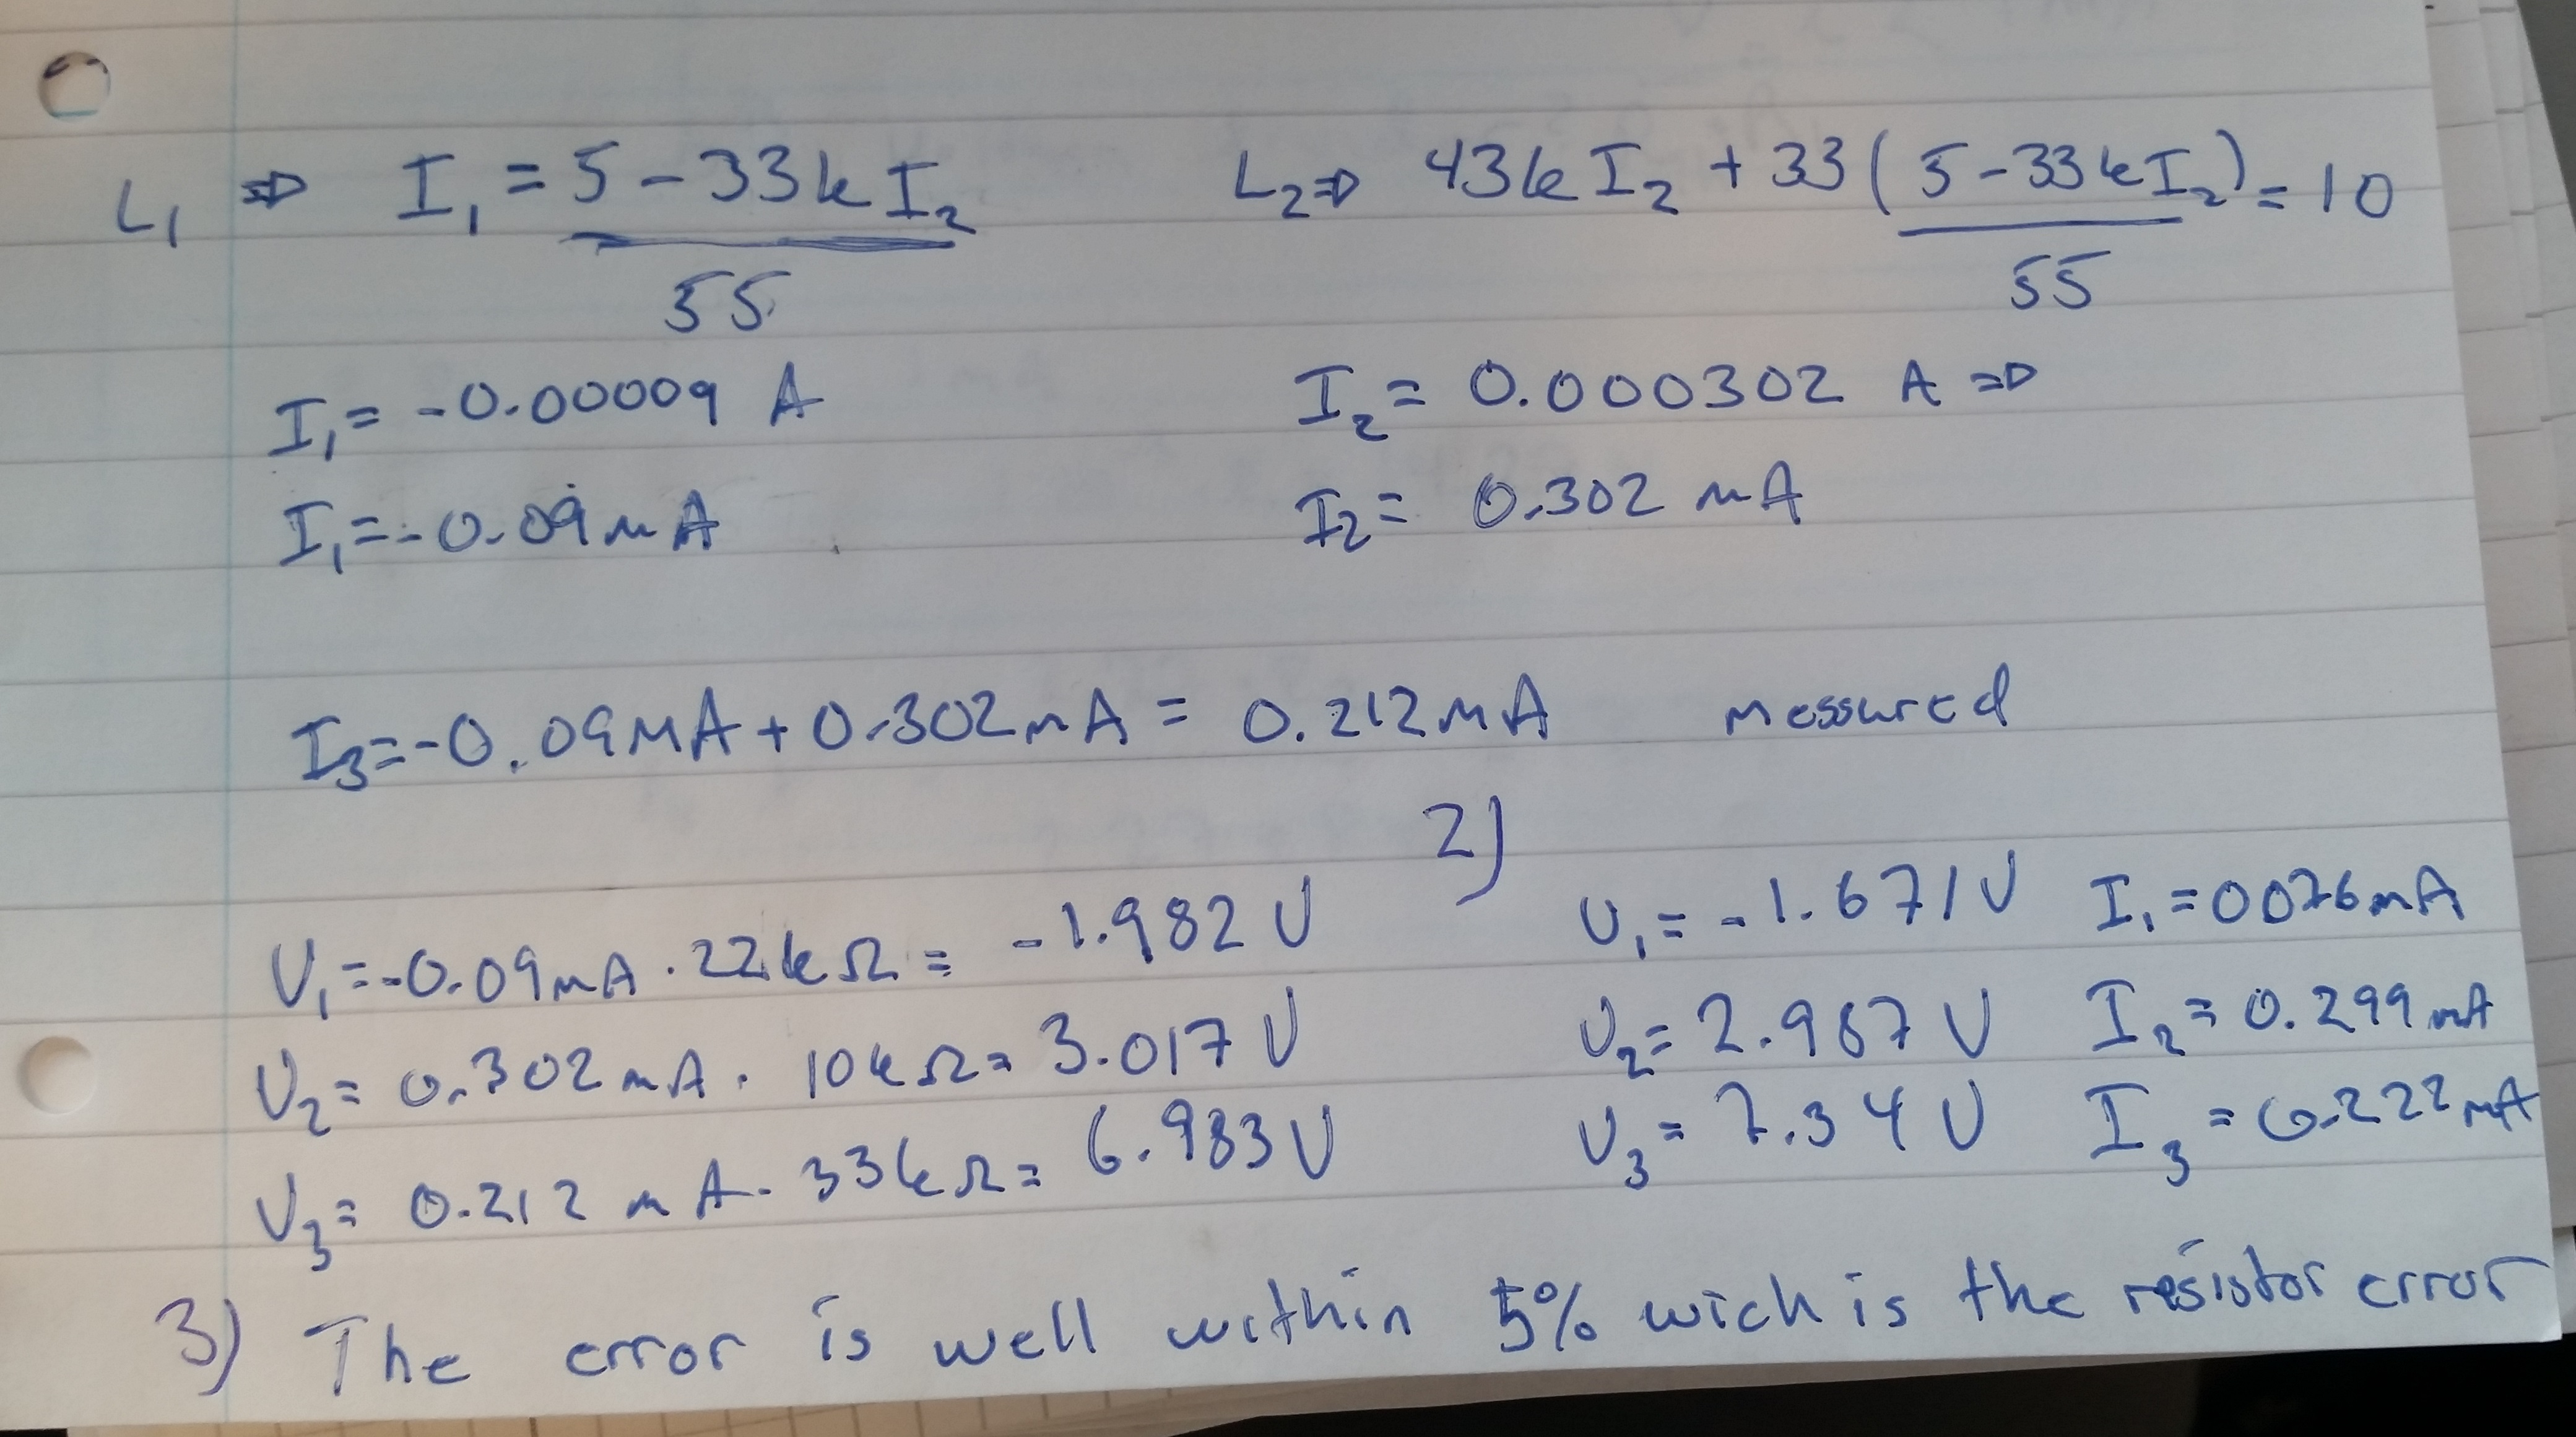
\includegraphics[width=0.6\textwidth]{images/lab1pic2.jpg}
		\end{figure}
	\end{solution}
	\clearpage	
	\begin{problem}
		Construct the circuit given in the following figure.
		\newline
		V\(_{A}\): 5V (with max current 60mA)\\
		I: 60mA (with max voltage 3V) \\
		R\(_{1}\): 180\(\Omega\) \\
		R\(_{2}\): 18\(\Omega\) \\
		R\(_{3}\): 270\(\Omega\) \\	
		\newline
		1. Calculate the voltage that falls on R\(_{3}\) using superposition.
		\newline
		2. Measure the voltage on R\(_{3}\).
		\newline
		3. Implement superposition in practice, by two tests (setting each source to zero and measuring the voltage)
		\newline
		4. Compare the results with your calculation.
		\newline
		5. Use the following resistors and explain why the measurements are not consistent with calculations\\
		R\(_{1}\): 180K\(\Omega\) \\
		R\(_{2}\): 18K\(\Omega\) \\
		R\(_{3}\): 270K\(\Omega\) \\	
		\begin{figure}[h!]
			\centering
			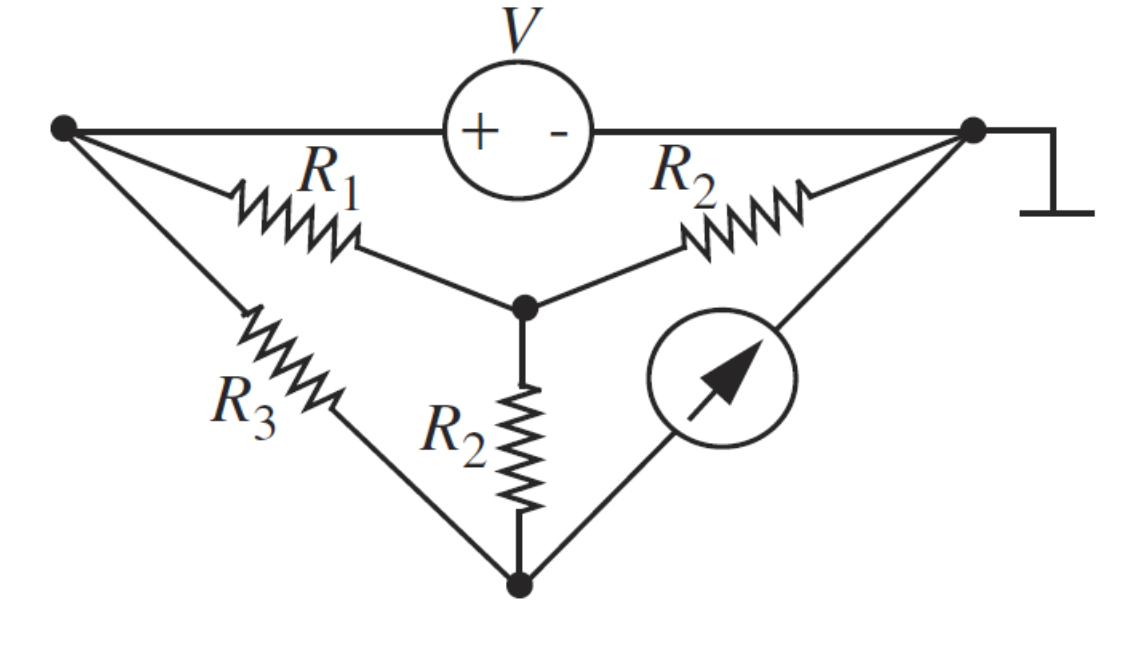
\includegraphics[width=0.3\textwidth]{images/circuit6.png}
		\end{figure}		
	\end{problem}
	
	\begin{solution}
		1.
		\begin{figure}[h!]
			\begin{subfigure}[H]{0.5\textwidth}
				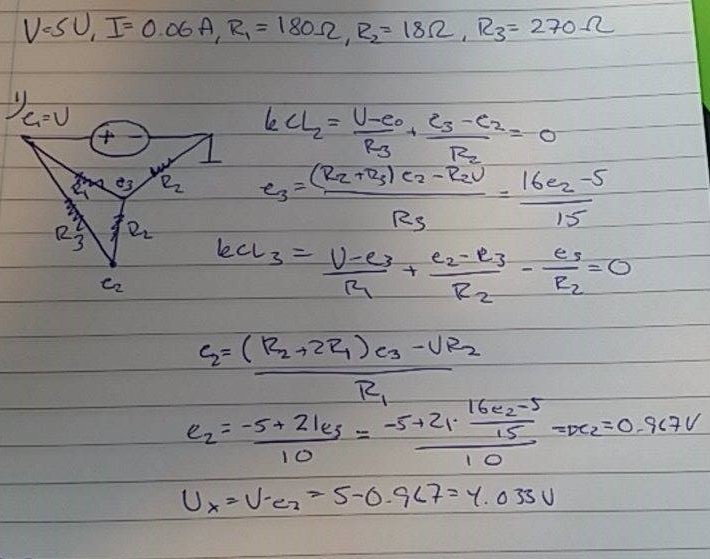
\includegraphics[width=0.8\textwidth]{images/lab3pic1.jpg}
				\subcaption{1.4.1}
			\end{subfigure}
			\begin{subfigure}[H]{0.7\textwidth}
				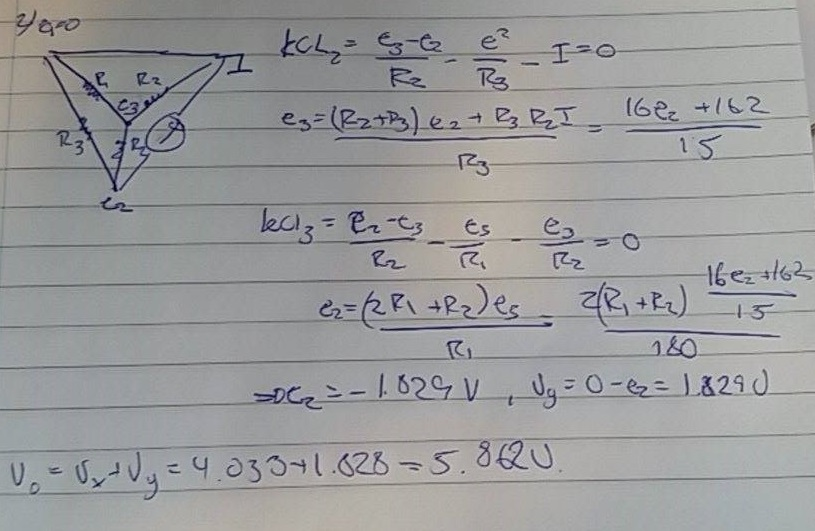
\includegraphics[width=0.7\textwidth]{images/lab3pic2.jpg}
				\subcaption{1.4.2}
			\end{subfigure}
		\end{figure}
		\newline
		2. R3= 5.59V
		\newline
		3. V1= 5.52, V2= 6mV, Total V= 5.58V
		\newline
		4. We calculated it to be 5.862V and measured it to be 5.8V.
		\newline
		5. I measured 8 V and said that the inconsistency is because in order to reach 60mA, we need a big voltage, so the current source reaches it's voltage limit and acts as a 3V voltage source.
	\end{solution}